\documentclass[12pt]{article}
\usepackage[margin=1in]{geometry}
\usepackage{setspace}
\usepackage{listings}
\usepackage[dvipsnames,table,xcdraw]{xcolor} % colors
\onehalfspacing{}

% Start of preamble
%==========================================================================================%
% Required to support mathematical unicode
\usepackage[warnunknown, fasterrors, mathletters]{ucs}
\usepackage[utf8x]{inputenc}
%\usepackage{R:/sty/quiver}

\usepackage{hyperref} % links
\hypersetup{
colorlinks=true,
linkcolor=blue,
filecolor=magenta,
urlcolor=cyan,
pdfpagemode=FullScreen
}

\definecolor{dkgreen}{rgb}{0,0.6,0}
\definecolor{gray}{rgb}{0.5,0.5,0.5}
\definecolor{mauve}{rgb}{0.58,0,0.82}

\lstset{frame=tb,
  language=Java,
  aboveskip=3mm,
  belowskip=3mm,
  showstringspaces=false,
  columns=flexible,
  basicstyle={\small\ttfamily},
  numbers=none,
  numberstyle=\tiny\color{gray},
  keywordstyle=\color{blue},
  commentstyle=\color{dkgreen},
  stringstyle=\color{mauve},
  breaklines=true,
  breakatwhitespace=true,
  tabsize=3
}



% Standard mathematical typesetting packages
\usepackage{amsmath,amssymb,amscd,amsthm,amsxtra, pxfonts}
\usepackage{mathtools,mathrsfs,xparse}

% Symbol and utility packages
\usepackage{cancel, textcomp}
\usepackage[mathscr]{euscript}
\usepackage[nointegrals]{wasysym}
\usepackage{apacite}

% Extras
\usepackage{physics}  % Lots of useful shortcuts and macros
\usepackage{tikz-cd}  % For drawing commutative diagrams easily
\usepackage{microtype}  % Minature font tweaks
%\usepackage{pgfplots} % plots

\usepackage{enumitem}
\usepackage{titling}

\usepackage{graphicx}

%\usepackage{quiver}

% Fancy theorems due to @intuitively on discord
\usepackage{mdframed}
\newmdtheoremenv[
backgroundcolor=NavyBlue!30,
linewidth=2pt,
linecolor=NavyBlue,
topline=false,
bottomline=false,
rightline=false,
innertopmargin=10pt,
innerbottommargin=10pt,
innerrightmargin=10pt,
innerleftmargin=10pt,
skipabove=\baselineskip,
skipbelow=\baselineskip]{mytheorem}{Theorem}

\newenvironment{theorem}{\begin{mytheorem}}{\end{mytheorem}}

\newtheorem{corollary}{Corollary}
\newtheorem{lemma}{Lemma}

\newtheoremstyle{definitionstyle}
{\topsep}%
{\topsep}%
{}%
{}%
{\bfseries}%
{.}%
{.5em}%
{}%
\theoremstyle{definitionstyle}
\newmdtheoremenv[
backgroundcolor=Violet!30,
linewidth=2pt,
linecolor=Violet,
topline=false,
bottomline=false,
rightline=false,
innertopmargin=10pt,
innerbottommargin=10pt,
innerrightmargin=10pt,
innerleftmargin=10pt,
skipabove=\baselineskip,
skipbelow=\baselineskip,
]{mydef}{Definition}
\newenvironment{definition}{\begin{mydef}}{\end{mydef}}

\newtheorem*{remark}{Remark}

\newtheorem*{example}{Example}
\newtheorem*{claim}{Claim}

% Common shortcuts
\def\mbb#1{\mathbb{#1}}
\def\mfk#1{\mathfrak{#1}}

\def\bN{\mbb{N}}
\def\C{\mbb{C}}
\def\R{\mbb{R}}
\def\bQ{\mbb{Q}}
\def\bZ{\mbb{Z}}
\def\cph{\varphi}
\renewcommand{\th}{\theta}
\def\ve{\varepsilon}
\newcommand{\mg}[1]{\| #1 \|}

% Often helpful macros
\newcommand{\floor}[1]{\left\lfloor#1\right\rfloor}
\newcommand{\ceil}[1]{\left\lceil#1\right\rceil}
\renewcommand{\qed}{\hfill\qedsymbol}
\renewcommand{\ip}[1]{\langle#1\rangle}
\newcommand{\seq}[2]{\qty(#1_#2)_{#2=1}^{\infty}}

\newcommand{\SET}[1]{\Set{\mskip-\medmuskip #1 \mskip-\medmuskip}}

% End of preamble
%==========================================================================================%

% Start of commands specific to this file
%==========================================================================================%

\usepackage{braket}
\newcommand{\Z}{\mbb Z}
\newcommand{\gen}[1]{\left\langle #1 \right\rangle}
\newcommand{\nsg}{\trianglelefteq}
\newcommand{\F}{\mbb F}
\newcommand{\Aut}{\mathrm{Aut}}
\newcommand{\sepdeg}[1]{[#1]_{\mathrm{sep}}}
\newcommand{\Q}{\mbb Q}
\newcommand{\Gal}{\mathrm{Gal}\qty}
\newcommand{\id}{\mathrm{id}}
\newcommand{\Hom}{\mathrm{Hom}_R}
\usepackage{float}
\newcommand{\E}{\mathbb E}

%==========================================================================================%
% End of commands specific to this file

\title{Optimal Matrices}
\date{\today}
\author{Rohan Mukherjee}

\begin{document}
    \maketitle
    \begin{theorem}[The center of the cube is the center of the cube]
        The unique vector $a \in \R^n$ minimizing 
        \begin{align*}
            f(a) = \frac{1}{2^n} \sum_{x \in \SET{\pm 1}^n} \mg{x-a}
        \end{align*} is just $a = 0$.
    \end{theorem}
    \begin{lemma}[Average of two points]
        Let $a \neq b \in \R^n$. The vectors minimizing 
        \begin{align*}
            f(x) = \frac12(\mg{x-a} + \mg{x-b})
        \end{align*}
        are $x = \lambda a + (1-\lambda)b$ for $0 \leq \lambda \leq 1$.
    \end{lemma}
    \begin{proof}
        Euclidean geometry.
    \end{proof}
    \begin{proof}[Proof of Hypercube Center]
        By the previous theorem, the minimizer between two opposite points of the cube $z, -z$ for $z \in \SET{-1,1}^n$ is attained on the line segment from $-z$ to $z$. The intersection of all these line segments is just $0$, so we are done, since we can partition our sum into $2^{n-1}$ pairs of opposite points, and we attain the minimum of each of these sums simultaneously. The author notes that this proof generalizes immediately to any regular polytope where the diagonals intersect in the origin.
    \end{proof}

    \begin{theorem}[Procedure for finding optimal matrices]
        Define
        \begin{align*}
            \beta(A) \coloneqq \sum_{x \in \SET{\pm 1}^n} \mg{Ax}_\infty
        \end{align*}        
        The maximum of $\beta(A)$ is attained (non-uniquely) via the following procedure:

        Define the set $C$ to be the boundary of the convex hull of the points $\SET{\pm 1}^{n-1} \times \SET{1}$, and let $F(a)$ for a point $a \in C$ to be the face that $a$ lies in the interior of, and let $G(a)$ be the set of faces of minimal dimension containing $F(a)$ as boundary (i.e., the link). Given the optimal $m \times n$ matrix attained from this procedure, the optimal $m-1 \times n$ matrix is obtained by finding two rows $a_1, a_2$ of $A$ minimizing the dimension of $F(a_1)=F(a_2)$ with $G(a_1) = G(a_2)$, and replacing them with their average.
    \end{theorem}

    I believe the above theorem can be restated using the defintions of cubical complexes more concisely. Also, my use of interior above is not the strict topological sense, but instead not lying on the boundary when looked at in the right dimension.

    \begin{proof}[Proof Ideas]
        I believe the proof would go something as follows. Either you start with the optimal $m \times n$ matrix and you show that the optimal $m-1 \times n$ matrix is obtained by the above procedure, then repeat using a "greedy stays ahead" type argument. 

        Another set of ideas I had was as follows:

        Since the infinity norm is invariant under the transformation $x \to -x$, we only have to maximize over the set of $x \in \SET{\pm 1}^n$ with the last coordinate being positive.

        Since $|c^2| = |a^2|+|b^2| - 2\ip{a,b}$, instead of maximizing the inner product we can minimize the distance, and normalize afterwards.

        Show that it is optimal to give each of the $m$ rows of $A$ disjoint subsets of the $2^{n-1}$ vertices of the hypercube $\SET{\pm 1}^{n-1} \times \SET{1}$, where each of these $m$ subsets has size a power of 2.

        The above might be shown by AM-GM, using that the average is minimized when all the points have equal distiance to the $a$th row. Somehow, the only possible way to have all the coordinates equal in distance to their geometric median is if they all have the same $G(\cdot)$ (this claim doesn't seem like it would be that hard).

        If there are $2^k$ points with the same $G(\cdot)$, the simple average of the points is going to be the optimizer of expected distance to each point in the group. This follows immediately by theorem 1.

        Somehow, the expected distance from the origin to the $k$-dimensional hypercube is less than the $k+1$-dimensional hypercube. This will follow once we can show the expected distance to the $k$-dimensional hypercube is just $C\sqrt{k+1}$ for some constant $C$.

        Lastly, we want to have the fewest number of points being packed into each group to minimize our average distance. Somehow, this will relate to having 2 infinity balls of size differing by 1, and in the case where the number of rows is a power of 2, there will only be 1 infinity ball. This will be the final step in the proof and will show after some simplification that this is precisely what the above procedure does.
    \end{proof}

    Let us use this procedure to find the optimal $4 \times 4$ matrix. The picture is as follows:
    \begin{figure}[H]
        \centering
        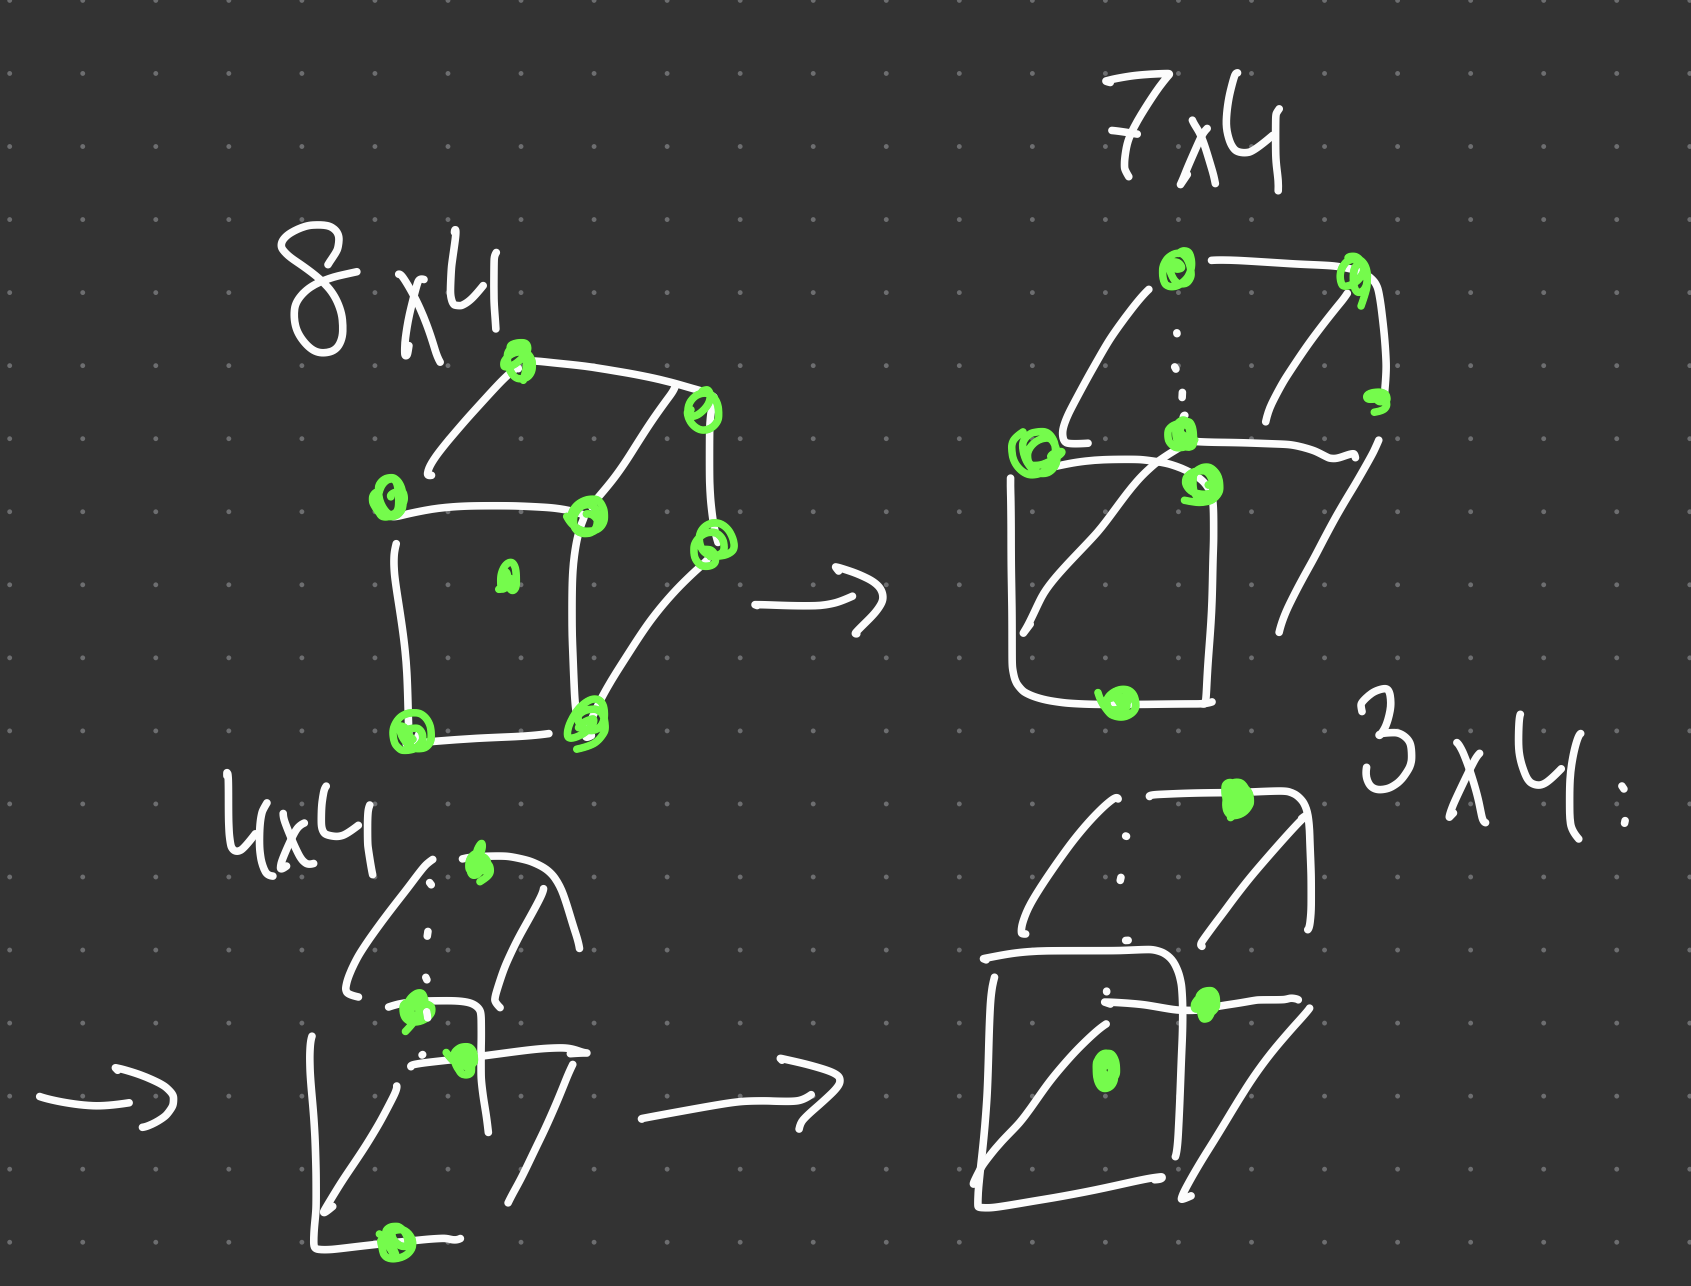
\includegraphics[width=0.7\textwidth]{opt4x4.png}
        \caption{Visualization of the Optimal 4x4 Matrix.}
        \label{fig: opt4x4}
    \end{figure}
    Notice that every time we take an average, we replace a $\pm 1$ in two rows with a 0 in one row. So, the matrices end up having many 0 entries, and when you take the averages in a systematic way, this translates to many columns of 0s. The matrix above is
    \begin{align*}
        \frac{1}{\sqrt{3}}\begin{pmatrix}
            1 & 1 & 0 & 1 \\
            1 & -1 & 0 & 1 \\
            -1 & 1 & 0 & 1 \\
            -1 & -1 & 0 & 1
        \end{pmatrix}
    \end{align*}

    For some intuition for why groups of powers of 2 are likely optimal, let's examine the $2 \times 3$ case. The optimal matrix is (very likely) 
    \begin{align*}
        \frac{1}{\sqrt{2}}\begin{pmatrix}
            1 & 0 & 1 \\
            -1 & 0 & 1
        \end{pmatrix}
    \end{align*}
    This corresponds to the following graph:
    \begin{figure}[H]
        \centering
        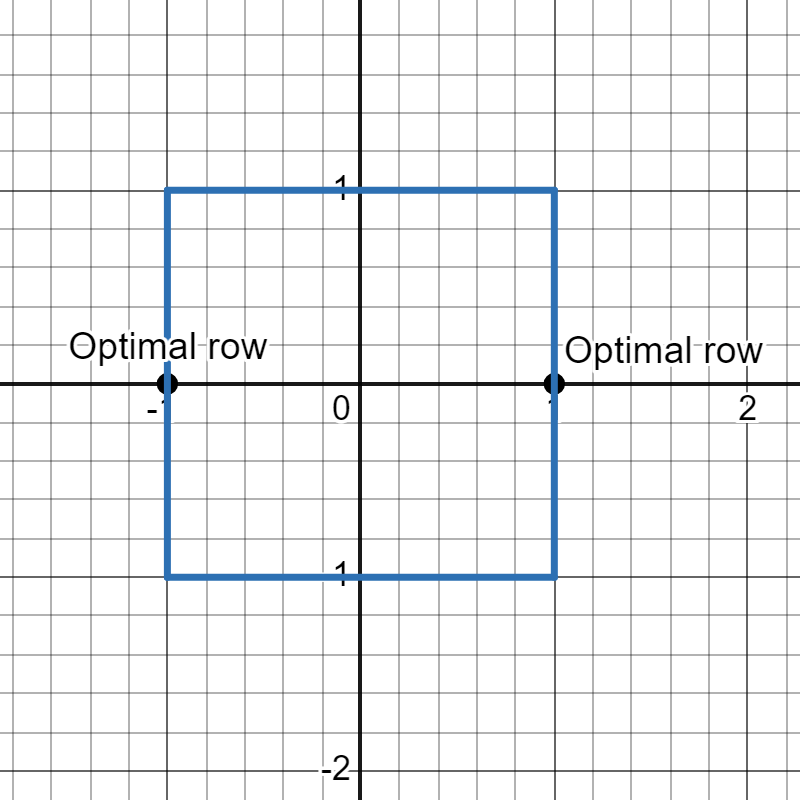
\includegraphics[width=0.45\textwidth]{opt2x3.png}
        \caption{Visualization of the Optimal 2x3 Matrix.}
        \label{fig: opt2x3}
    \end{figure}
    Where the two groups in this case are the vertices on the left edge and the vertices on the right edge. However, could non-powers of 2 work better? For example, if we had groups with 3 vertices and 1 vertex respectively, we would get the optimal matrix being:
    \begin{align*}
        \begin{pmatrix}
            -\frac13 & -\frac13 & 1 \\
            1 & 1 & 1
        \end{pmatrix}
    \end{align*}
    Corresponding to:
    \begin{figure}[H]
        \centering
        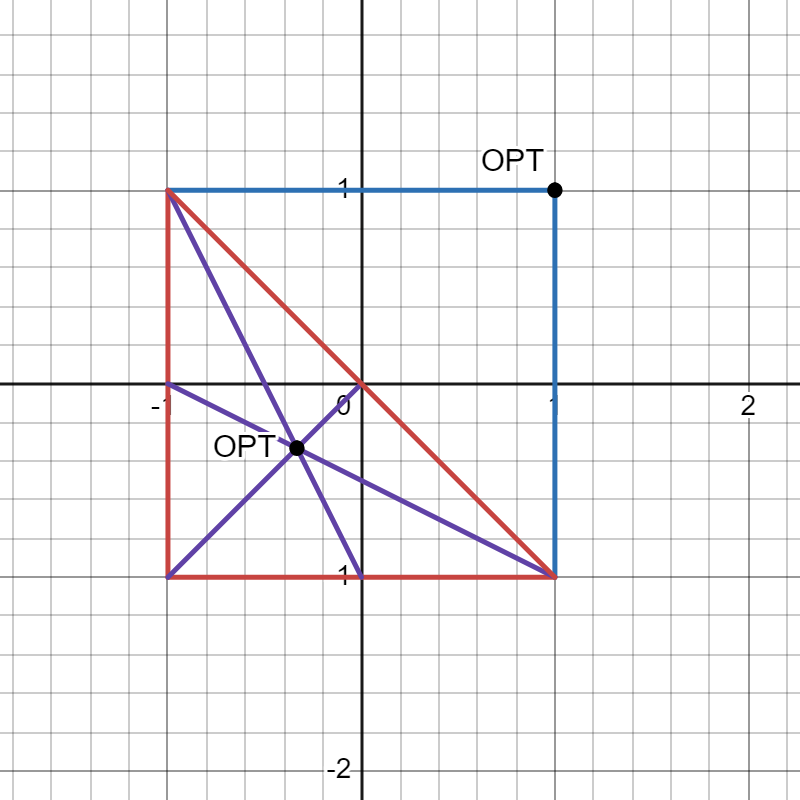
\includegraphics[width=0.45\textwidth]{opt3points.png}
        \caption{Visualization of the Optimal 2x3 Matrix with Non-Powers of 2.}
        \label{fig: opt2x3nonpow}
    \end{figure}
    This matrix has a beta value of around 1.262 which is far less than $\sqrt{2}$. The reason for this is because the geometric median of the triangle gives far too much weight to the bottom left point (around 1.5), while it only gives 0.9 weight to the top left / bottom right points. Lukshya and I believe this is related to \href{https://math.stackexchange.com/questions/3966303/evenly-distributing-n2-ball-between-n-pockets-by-chosing-2-of-them-at-a-t}{this} stack exchange post.

    An immediate consequence of this construction is to find (likely) optimal beta values for $2^k \times n$ matrices for $n > k$. For example, the optimal $4 \times 4$ we found above is:
    \begin{align*}
        O = \frac{1}{\sqrt{3}}\begin{pmatrix}
            1 & 1 & 0 & 1 \\
            1 & -1 & 0 & 1 \\
            -1 & 1 & 0 & 1 \\
            -1 & -1 & 0 & 1
        \end{pmatrix}
    \end{align*}
    With $\beta(O) = \sqrt{3}$. This construction obviously generalizes and one can see the optimal $2^k \times n$ matrix for $n > k$ has a $\beta$ value of at least (and likely exactly) $\sqrt{k+1}$. Optimal $2^n \times 2^n$ matrices can be found using the following line of code:
    \begin{lstlisting}[language=Python]
        A = np.c_[np.c_[np.array(list(it.product([-1,1], repeat=n))), np.zeros((2**n, 2**n-n-1))], np.ones((2**n, 1))]
    \end{lstlisting}
    

    A consequence of my construction is that the (likely) optimal beta value always takes the form
    \begin{align*}
        \beta(A) = \frac{a\sqrt{k} + b\sqrt{k+1}}{2^{n-1}}
    \end{align*}
    with $a+b=2^{n-1}$. This is because the above procedure clearly puts the vertices of the hypercube on two infinity balls with the expected inner product being $\sqrt{k}$ and $\sqrt{k+1}$ respectively, and since it puts the vertices into disjoint groups, we get the above form. So powers of 2 are special in the sense that the optimal matrix can pack all the points on one infinity ball, but there is even more going on behind the scenes (and in fact I like to describe this as discretely interpolating between $\sqrt{k}$ and $\sqrt{k+1}$ when the number of rows are between $2^{k-1}$ and $2^k$).

    Robert has proved that $n \times 1$ is tight in the following way:

    Recall that we can reformulate our problem using probability by showing that 
    \begin{align*}
        \E_x[|a^t x|] \leq 1
    \end{align*}
    Where $x$ is uniformly distributed on $\SET{\pm 1}^n$. Notice that 
    \begin{align*}
        (xx^t)_{ij} = x_i x_j
    \end{align*}
    And thus $\E[xx^t] = I$ by independence. Then,
    \begin{align*}
        \E[\ip{a,x}^2] = a^t \E[xx^t] a = a^t a = \mg{a}^2
    \end{align*}
    By Jensens,
    \begin{align*}
        \E[|a^t x|] = \E[\sqrt{\ip{a,x}^2}] \leq \sqrt{\E[\ip{a,x}^2]} = \mg{a} = 1
    \end{align*}
\end{document}